\documentclass{standalone}
%<--------------------------------------------------------------------------->%
%%% TikZ %%%
\usepackage{tikz}
% \usetikzlibrary{calc}
% \usetikzlibrary{angles,quotes}
% \usetikzlibrary{intersections,topaths}
% \usetikzlibrary{decorations.markings}
%<--------------------------------------------------------------------------->%

\begin{document}

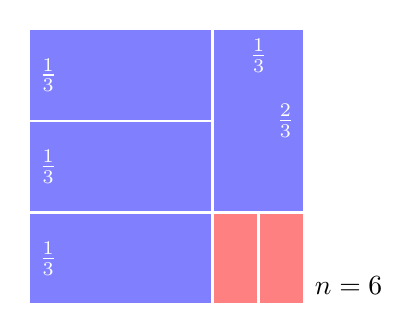
\begin{tikzpicture}[scale=3.5,thick,line cap=round,yscale=-1]
	\tikzstyle{jiao}=[solid,circle,draw,fill=white,inner sep=.8pt];
	\tikzstyle{tile1}=[line width=0.1em,draw=white,fill=blue!50];
\tikzstyle{tile2}=[line width=0.1em,draw=white,fill=red!50];
\tikzstyle{tile3}=[line width=0.1em,draw=white,fill=blue!50!red!60];
\tikzstyle{tile4}=[line width=0.1em,draw=white,fill=blue!20!red!60];

	\draw[tile1] (0,0)     rectangle (2/3,1/3);
	\draw[tile1] (0,1/3)   rectangle (2/3,2/3);
	\draw[tile1] (0,2/3)   rectangle (2/3,1);
	\draw[tile1] (2/3,0)   rectangle (1,2/3);
	\draw[tile2] (2/3,2/3) rectangle (5/6,1);
	\draw[tile2] (5/6,2/3) rectangle (1,1);
	\node[white,right] at (0,1/6) {$\frac{1}{3}$};
	\node[white,right] at (0,3/6) {$\frac{1}{3}$};
	\node[white,right] at (0,5/6) {$\frac{1}{3}$};
	\node[white,below] at (5/6,0) {$\frac{1}{3}$};
	\node[white,left] at (1,1/3) {$\frac{2}{3}$};
	\node[above right] at (1,1) {$n=6$};
\end{tikzpicture}

\end{document}

